\documentclass[12pt]{article}

\usepackage[a4paper,margin=1in]{geometry}
\usepackage[T1]{fontenc}
\usepackage[utf8]{inputenc}
\usepackage{lmodern}
\usepackage{setspace}
\usepackage{graphicx}
\usepackage{booktabs}
\usepackage{array}
\usepackage{amsmath}
\usepackage{hyperref}
\usepackage{float}

\setstretch{1.15}

\title{Assignment 4 Report: Sharding of the Developed Application}
\author{}
\date{}

\begin{document}

\maketitle

\section*{Submission Metadata}
\begin{itemize}
    \item GitHub Repository Link: \url{https://github.com/jsmaskeen/CS432-Assignments}
    \item Video Demonstration Link: \url{https://youtu.be/nFx1wKIRPDM}
    \item Course: CS 432 Databases
    \item Assignment: Track 1 Assignment 4
\end{itemize}

\hrule
\vspace{0.75em}

\section{Objective}

We extend the existing ride-sharing backend with horizontal scaling through sharding. The idea is to split ride-centric data across three shards and route requests correctly while preserving consistency of business logic and acceptable query latency.

We explain the below in this report:
\begin{enumerate}
    \item Shard key selection and justification.
    \item Data partitioning and migration into at least three shards.
    \item Query routing for lookups, inserts, and range-style access patterns.
    \item Scalability and trade-off analysis (consistency, availability, partition tolerance).
\end{enumerate}

\hrule
\vspace{0.75em}

\section{Environment}

\subsection{Shard Simulation Approach Used}

The system uses multiple databases on the same server (simulated independent shard nodes), configured as:
\begin{itemize}
    \item shard 0: port 3307
    \item shard 1: port 3308
    \item shard 2: port 3309
\end{itemize}

Shard engines and session factories are defined in \texttt{backend/db/sharding.py}.

\subsection{How Shard Isolation is Achieved}

The implementation uses multiple databases (not Docker containers) to represent independent shard nodes.
Isolation is enforced by architecture and connection boundaries:
\begin{itemize}
    \item Each shard has a dedicated SQLAlchemy engine and session factory bound to its own host/port.
    \item Single-ride requests resolve one \texttt{ShardID} and execute only on that shard session.
    \item Cross-shard reads are explicit fan-out operations (query each shard, then merge), rather than implicit shared access.
    \item Metadata directories (\texttt{Ride\_Shard\_Directory}, range directory, review directory) remain in the primary metadata database, separate from ride-data shards.
\end{itemize}

\subsection{Pipeline}

The full pipeline was executed in order:
\begin{enumerate}
    \item Cleanup/reset from SQL dump.
    \item Large fake data generation.
    \item Dry-run migration verification.
    \item Actual migration to shards.
    \item Post-migration validation.
    \item Benchmarking shard lookup strategies (baseline and range-enabled).
    \item Entropy-based shard-key analysis.
    \item Distribution figure generation.
\end{enumerate}

\subsection{Dataset Size Used for Final Evaluation}

\begin{itemize}
    \item \texttt{rides\_total}: 6000
    \item \texttt{bookings\_total}: 13370
    \item \texttt{shard\_count}: 3
\end{itemize}

\hrule
\vspace{0.75em}

\section{SubTask 1: Shard Key Selection and Justification}

\subsection{Selection Criteria}

The selected shard key should satisfy:
\begin{enumerate}
    \item High cardinality
    \item Query alignment
    \item Stability after insertion
\end{enumerate}

\subsection{Partitioning Strategy Families}

Before selecting a shard key formula, we evaluated all three strategy families required by the assignment.

\subsubsection*{A) Range-Based Partitioning}

Definition: Key ranges are assigned to shard IDs (for example, 1--2000 to shard 0, 2001--4000 to shard 1, and 4001+ to shard 2).

What we implemented:
\begin{itemize}
    \item Range-rule support via \texttt{Ride\_Shard\_Range\_Directory} (a metadata table that stores \texttt{MinRideID}, \texttt{MaxRideID}, and target \texttt{ShardID}) and the configuration script.
    \item Runtime evaluation support through \texttt{directory\_range} lookup mode (router checks range rules first to pick shard) and strategy benchmarking.
\end{itemize}

Advantages:
\begin{itemize}
    \item Easy to reason about and debug.
    \item Useful for planned archival tiers and batch movement by key intervals.
\end{itemize}

Limitations:
\begin{itemize}
    \item Can drift into skew as real insert/update patterns change.
    \item Requires operational maintenance of ranges and rebalancing rules.
\end{itemize}

\subsubsection*{B) Hash-Based Partitioning}

Definition:
\begin{itemize}
    \item Compute shard by a deterministic function of a key, then modulo by shard count.
\end{itemize}

What we implemented:
\begin{itemize}
    \item Deterministic modulo on RideID: \texttt{shard\_id = (RideID - 1) \% 3} (same input RideID always maps to the same shard without any directory lookup).
    \item Additional hashed candidates for analysis (geohash, vehicle type, status, composite keys) where \texttt{md5(value) \% 3} is used to test balance quality.
\end{itemize}

Advantages:
\begin{itemize}
    \item Very low lookup overhead.
    \item Good statistical balance when key domain is suitable.
    \item No metadata lookup required during request routing.
\end{itemize}

Limitations:
\begin{itemize}
    \item Harder to force special placement for specific keys without additional directory layer.
\end{itemize}

\subsubsection*{C) Directory-Based Partitioning}

Definition:
\begin{itemize}
    \item A lookup directory maps keys (or ranges) to shards explicitly.
\end{itemize}

What we implemented:
\begin{itemize}
    \item Exact directory: \texttt{Ride\_Shard\_Directory} (one row per \texttt{RideID}, explicit mapping \texttt{RideID -> ShardID}).
    \item Range directory: \texttt{Ride\_Shard\_Range\_Directory} (one row per key interval, mapping \texttt{RideID range -> ShardID}).
\end{itemize}

Advantages:
\begin{itemize}
    \item Flexible placement and migration control.
    \item Useful for overrides, controlled movement, and operational tooling.
\end{itemize}

Limitations:
\begin{itemize}
    \item Extra metadata dependency for routing.
    \item Slightly higher lookup overhead versus pure deterministic modulo.
\end{itemize}

\subsubsection*{Strategy-Level Outcome}

All three families were implemented and we compared the three routing families.

Strategy-family outcome tables:

Baseline run (no range rules):

\begin{table}[H]
\centering
\begin{minipage}{\textwidth}
\centering
\resizebox{\textwidth}{!}{%
\begin{tabular}{l l r r r r}
\toprule
Strategy Family & Concrete Strategy & Lookups/s & Avg (ms) & Normalized Entropy & Imbalance Spread \\
\midrule
Hash-based & modulo & 1,979,041.95 & 0.000234 & 0.999938 & 190 \\
Directory-based & directory\_exact\_cache & 1,154,054.77 & 0.000520 & 0.999885 & 257 \\
\bottomrule
\end{tabular}%
}
\end{minipage}
\end{table}

Range-enabled run (3 range rules active):

\begin{table}[H]
\centering
\begin{minipage}{\textwidth}
\centering
\resizebox{\textwidth}{!}{%
\begin{tabular}{l l r r r r}
\toprule
Strategy Family & Concrete Strategy & Lookups/s & Avg (ms) & Normalized Entropy & Imbalance Spread \\
\midrule
Hash-based & modulo & 2,079,391.15 & 0.000223 & 0.999938 & 190 \\
Directory-based (exact) & directory\_exact\_cache & 1,453,794.77 & 0.000402 & 0.999885 & 257 \\
Range-directory & directory\_range\_cache & 1,462,800.97 & 0.000438 & 0.999960 & 138 \\
\bottomrule
\end{tabular}%
}
\end{minipage}
\end{table}

Decision from these outcomes:
\begin{enumerate}
    \item Hash-based modulo gives the highest lookup throughput in both runs.
    \item Range-directory can improve sampled distribution compactness (lower spread), but routing overhead remains higher than modulo.
    \item Therefore, the runtime default remains deterministic hash-based modulo, while directory exact/range are retained as operational tools for migration and future rebalance controls.
\end{enumerate}

\subsection{Candidate Shard Keys Evaluated Under Hash-Based Mapping}

The implementation does not rely on only one trial. It evaluates multiple candidate policies:
\begin{itemize}
    \item ride\_id\_mod3: (RideID - 1) \% 3
    \item host\_member\_id\_mod3: (Host\_MemberID - 1) \% 3
    \item start\_geohash\_hash: md5(Start\_GeoHash) \% 3
    \item end\_geohash\_hash: md5(End\_GeoHash) \% 3
    \item vehicle\_type\_hash: md5(Vehicle\_Type) \% 3
    \item ride\_status\_hash: md5(Ride\_Status) \% 3
    \item host\_plus\_start\_hash: md5(Host\_MemberID|Start\_GeoHash) \% 3
    \item route\_pair\_hash: md5(Start\_GeoHash|End\_GeoHash) \% 3
\end{itemize}

How to read these candidate names:
\begin{itemize}
    \item \texttt{ride\_id\_mod3}: take \texttt{RideID}, apply modulo 3.
    \item \texttt{host\_member\_id\_mod3}: take host member id, apply modulo 3.
    \item \texttt{*\_hash}: hash the selected field(s), then apply modulo 3.
    \item \texttt{host\_plus\_start\_hash}: hash of \texttt{Host\_MemberID} and \texttt{Start\_GeoHash} combined.
    \item \texttt{route\_pair\_hash}: hash of \texttt{(Start\_GeoHash, End\_GeoHash)} pair.
\end{itemize}

\subsection{Entropy Metric and Why It Matters}

To quantify shard balance quality, entropy over 3 shards is used:

\[
H = -\sum_{i=0}^{2} p_i\log_2(p_i),\qquad
H_{\max} = \log_2(3) \approx 1.5849625,
\]

\[
H_{\text{normalized}} = \frac{H}{H_{\max}}
\]

Where $p_i$ is the fraction of records mapped to shard $i$.

Interpretation:
\begin{itemize}
    \item $H_{\text{normalized}}$ close to 1.0 means near-perfect balance.
    \item $H_{\text{normalized}}$ close to 0 means severe skew (one shard dominates).
\end{itemize}

\subsection{Entropy Ranking Results on Final Dataset}

\begin{table}[H]
\centering
\begin{minipage}{\textwidth}
\centering
\resizebox{\textwidth}{!}{%
\begin{tabular}{l l l r r}
\toprule
Candidate & Method & Counts (0/1/2) & Normalized Entropy & Imbalance Spread \\
\midrule
ride\_id\_mod3 & (RideID - 1) \% 3 & 2000 / 2000 / 2000 & 1.000000 & 0 \\
route\_pair\_hash & md5(Start\_GeoHash\textbar End\_GeoHash) \% 3 & 2016 / 2003 / 1981 & 0.999976 & 35 \\
end\_geohash\_hash & md5(End\_GeoHash) \% 3 & 2038 / 1974 / 1988 & 0.999914 & 64 \\
start\_geohash\_hash & md5(Start\_GeoHash) \% 3 & 1949 / 2024 / 2027 & 0.999851 & 78 \\
host\_plus\_start\_hash & md5(Host\_MemberID\textbar Start\_GeoHash) \% 3 & 2031 / 1941 / 2028 & 0.999801 & 90 \\
host\_member\_id\_mod3 & (Host\_MemberID - 1) \% 3 & 2018 / 2063 / 1919 & 0.999587 & 144 \\
vehicle\_type\_hash & md5(Vehicle\_Type) \% 3 & 1478 / 1486 / 3036 & 0.942542 & 1558 \\
ride\_status\_hash & md5(Ride\_Status) \% 3 & 6000 / 0 / 0 & 0.000000 & 6000 \\
\bottomrule
\end{tabular}%
}
\end{minipage}
\end{table}

\subsection{Final Decision: Why RideID Modulo-3 Over Other Strategies}

The selected shard key is RideID with the deterministic mapping:

\texttt{shard\_id = (RideID - 1) \% 3}

This choice is justified by the criteria given and by comparison against the alternatives:

\begin{enumerate}
    \item Compared with range-based routing:
    \begin{itemize}
        \item Range policies are useful, but require ongoing rule maintenance and can skew as workload evolves.
        \item Deterministic modulo avoids rule computation and gives stable long-run behavior.
    \end{itemize}

    \item Compared with directory-exact as default routing:
    \begin{itemize}
        \item Directory-exact is excellent for migration/override control, but adds metadata lookup dependency to every route resolution.
        \item Modulo offers simpler and faster request-path routing.
    \end{itemize}

    \item Compared with other candidate hash keys:
    \begin{itemize}
        \item Non-RideID candidates can be balanced, but many are less query-aligned for ride-centric APIs.
        \item RideID is the dominant join and routing handle across rides, bookings, chat, reviews, and settlements.
    \end{itemize}

    \item Against the three key criteria:
\end{enumerate}

\textbf{High cardinality:}\\
RideID is unique and uniformly increasing, giving excellent spread.

\textbf{Query alignment:}\\
RideID is central in ride, booking, chat, review, and settlement flows. Many APIs directly include \texttt{ride\_id} path parameters.

\textbf{Stability:}\\
RideID is immutable after insert, which avoids re-sharding computation.

In the final measured dataset, this key reached perfect entropy balance and zero imbalance spread.

\subsection{Distribution Figure}

The generated figure comparing candidate policy distributions:

\begin{figure}[H]
    \centering
    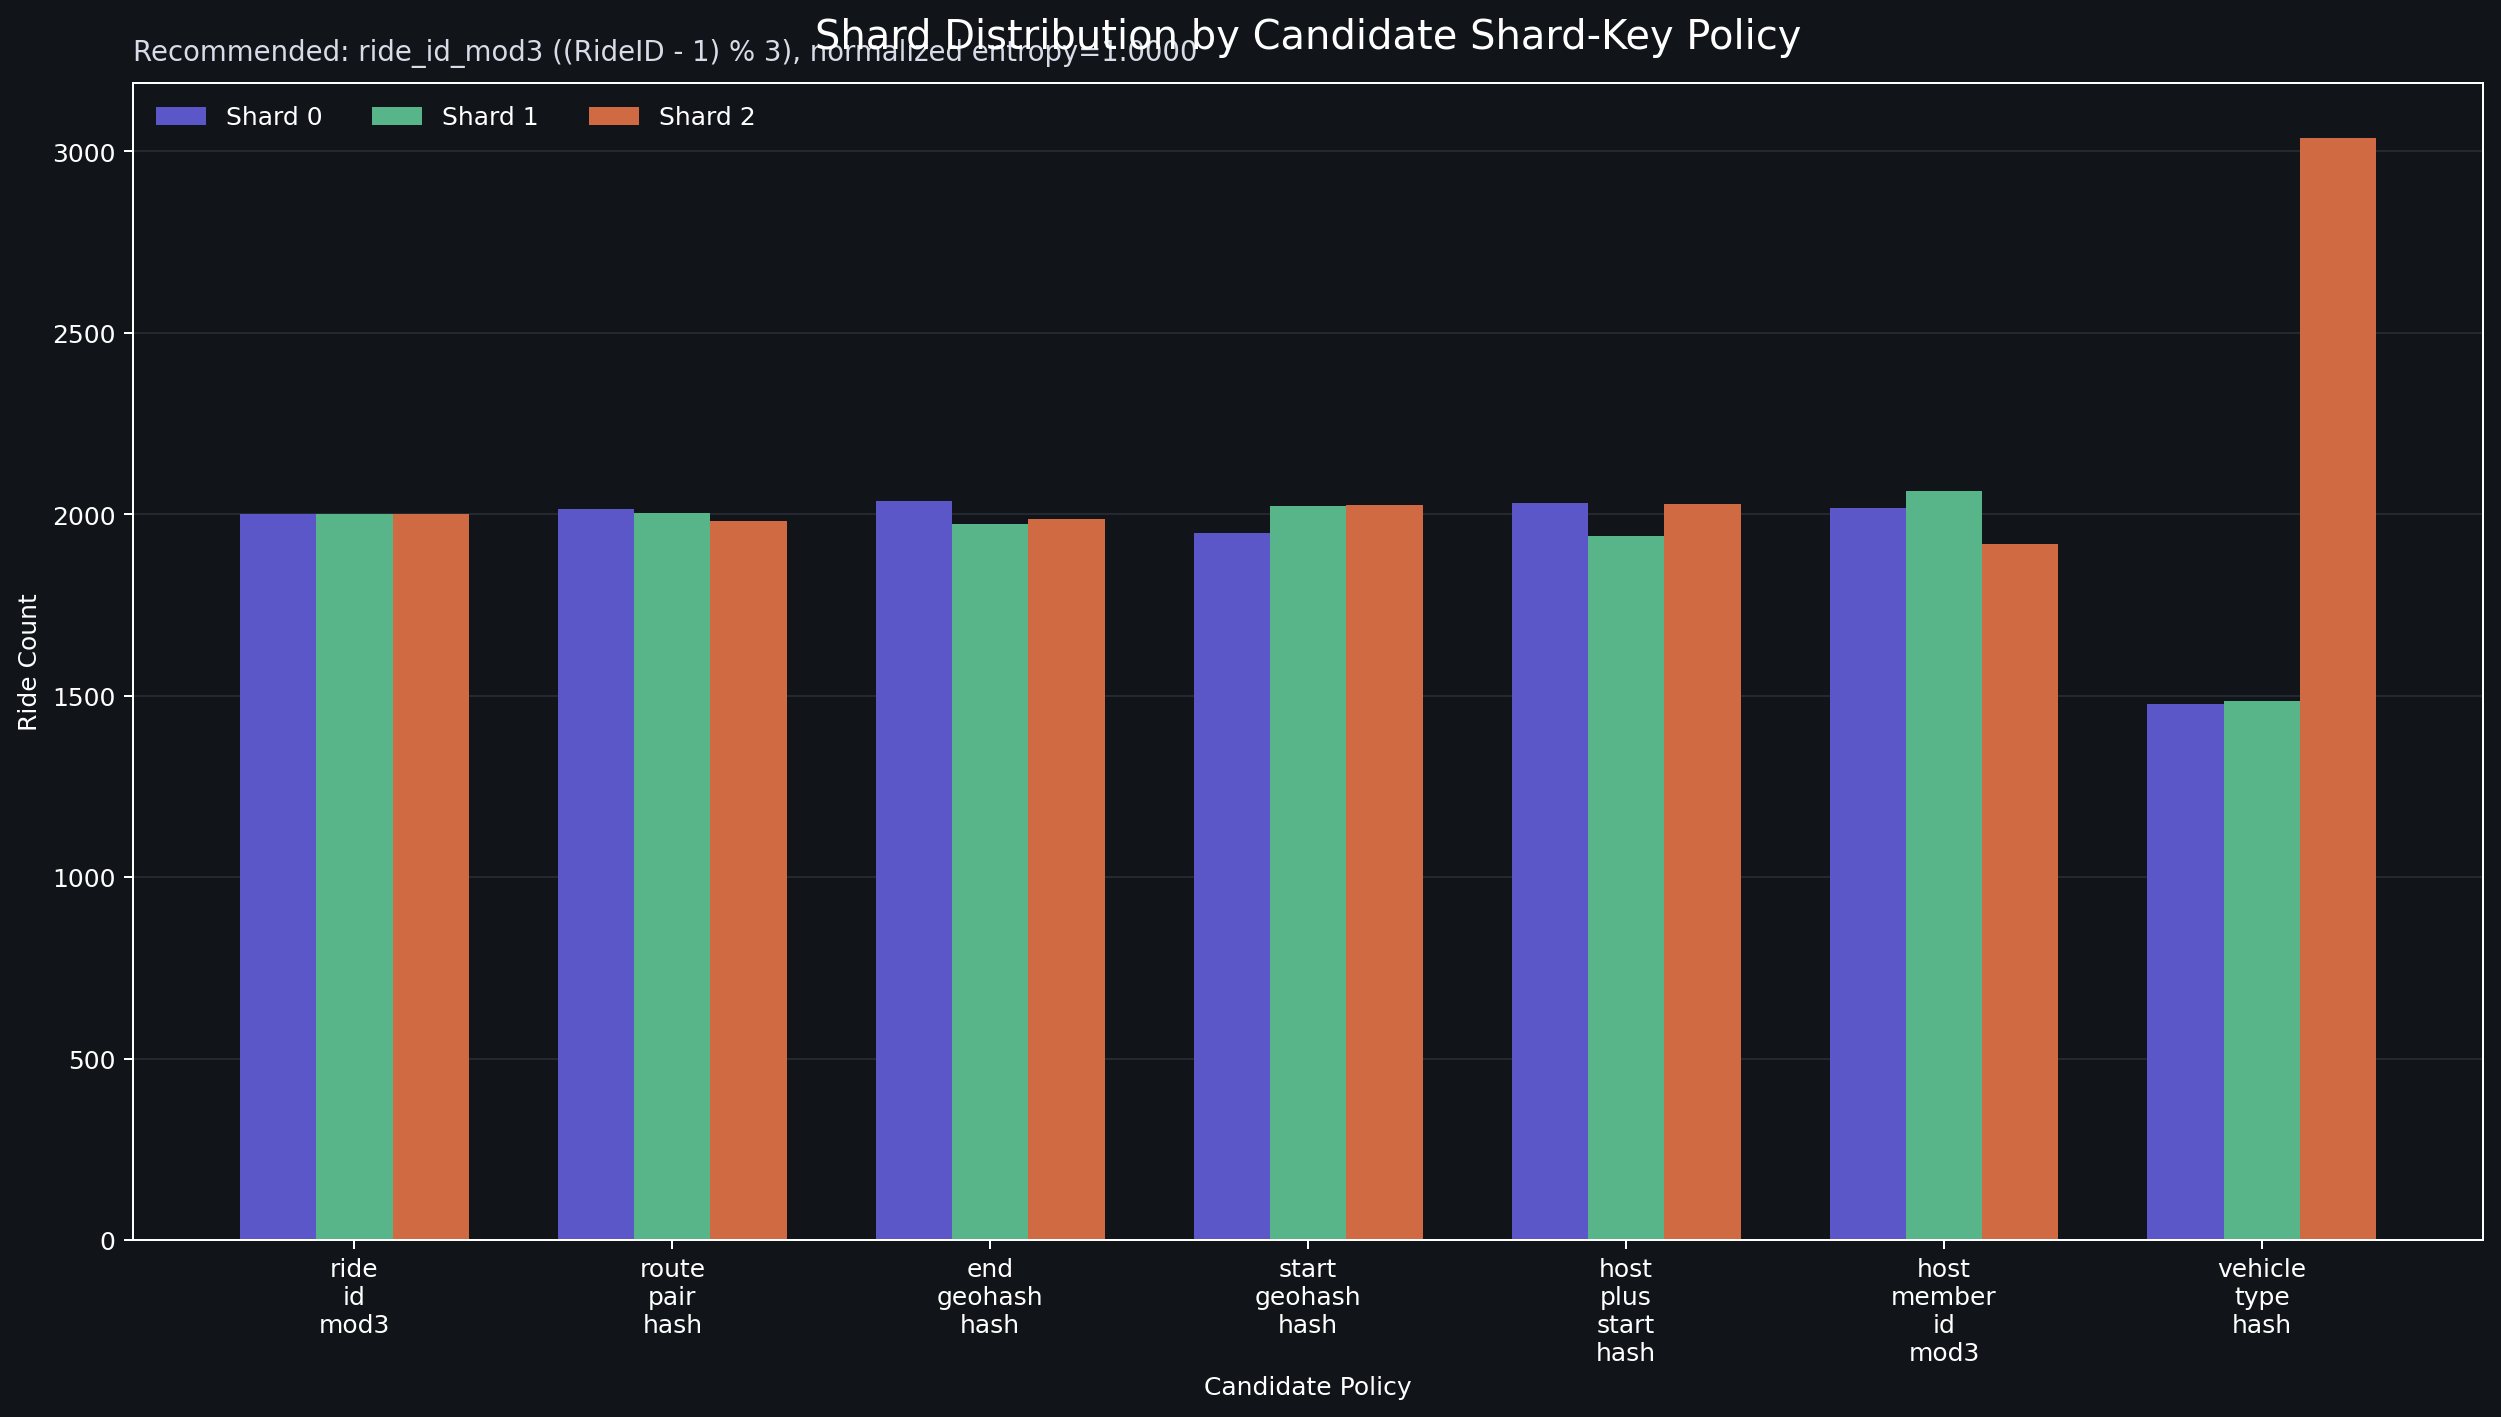
\includegraphics[width=0.9\textwidth]{../images/shard_key_policy_distribution.png}
    \caption{Shard distribution across candidate shard-key policies}
\end{figure}

This figure visually confirms the entropy table: RideID modulo-3 is perfectly balanced on the evaluated dataset.

\subsection{Relevant Code Snippet (Shard Function)}

\begin{verbatim}
def shard_id_for_ride_id(ride_id: int) -> int:
    if ride_id <= 0:
        raise ValueError(f"ride_id must be positive, got {ride_id}")
    return (ride_id - 1) % 3
\end{verbatim}

\hrule
\vspace{0.75em}

\section{SubTask 2: Implement Data Partitioning}

\subsection{Shard Tables and Data Layout}

Each shard database contains the physical SQL shard tables:
\begin{itemize}
    \item Members (mirrored subset needed for FK integrity)
    \item Rides
    \item Bookings
    \item Ride\_Chat
    \item Ride\_Participants
    \item Reputation\_Reviews
    \item Cost\_Settlements
\end{itemize}

Ride-centric rows were partitioned across all three shards:
\begin{itemize}
    \item Rides
    \item Bookings
    \item Ride\_Chat
    \item Ride\_Participants
    \item Reputation\_Reviews
    \item Cost\_Settlements
\end{itemize}

Supporting directory tables are maintained in the primary metadata database:
\begin{itemize}
    \item Ride\_Shard\_Directory
    \item Ride\_Shard\_Range\_Directory
    \item Review\_Shard\_Directory
\end{itemize}

\subsection{Migration Method Used}

The migration script \texttt{backend/scripts/migrate\_rides\_to\_shards.py}:
\begin{enumerate}
    \item Reads source ride-centric tables.
    \item Computes shard target by \texttt{shard\_id\_for\_ride\_id}.
    \item Builds shard-wise row buckets.
    \item Rebuilds per-shard data by clearing ride-centric rows first.
    \item Re-inserts Members required by shard FK constraints.
    \item Writes \texttt{Ride\_Shard\_Directory} for deterministic and directory-assisted routing.
\end{enumerate}

\subsection{Migration Validation and Integrity}

Current validation output (\texttt{backend/scripts/validate\_shard\_migration.py}):
\begin{itemize}
    \item \texttt{ride\_placement\_summary}: misplaced=0, duplicate=0, unique\_rides=6000
    \item \texttt{directory\_summary}: entries=6000, mismatches=0
\end{itemize}

These are the key correctness conditions: no misplaced rides, no duplicate ride IDs across shards, and directory consistency.

For this reason, ride placement and directory checks are the decisive integrity checks here, and they pass.

\subsection{Observed Final Per-Shard Data Distribution}

Measured after migration:

\begin{table}[H]
\centering
\begin{minipage}{\textwidth}
\centering
\resizebox{\textwidth}{!}{%
\begin{tabular}{l r r r r}
\toprule
Table & Shard 0 & Shard 1 & Shard 2 & Total \\
\midrule
Rides & 2000 & 2000 & 2000 & 6000 \\
Bookings & 4545 & 4396 & 4429 & 13370 \\
Ride\_Chat & 6000 & 6000 & 6000 & 18000 \\
Ride\_Participants & 4545 & 4396 & 4429 & 13370 \\
Reputation\_Reviews & 1642 & 1549 & 1618 & 4809 \\
Cost\_Settlements & 2545 & 2396 & 2429 & 7370 \\
\bottomrule
\end{tabular}%
}
\end{minipage}
\end{table}

The distribution for dependent ride-centric entities tracks the ride partitioning and generated activity per ride.

\subsection{Relevant Migration Snippet}

\begin{verbatim}
for ride in rides:
    shard_id = shard_id_for_ride_id(int(ride["RideID"]))
    shard_rows[shard_id]["Rides"].append(ride)
    directory_rows.append({
        "RideID": int(ride["RideID"]),
        "ShardID": shard_id,
        "Strategy": "ride_id_mod_3",
    })
\end{verbatim}

\hrule
\vspace{0.75em}

\section{SubTask 3: Implement Query Routing}

\subsection{Lookup Queries}

Single-key lookups resolve shard from \texttt{ride\_id} and query only the target shard.

Examples:
\begin{itemize}
    \item GET /api/v1/rides/\{ride\_id\}
    \item GET /api/v1/chat/ride/\{ride\_id\}
    \item GET /api/v1/reviews/ride/\{ride\_id\}
\end{itemize}

\subsection{Insert Operations}

Insert paths compute the target shard at write time, then:
\begin{enumerate}
    \item Persist core metadata and directory mapping.
    \item Persist ride-centric row set to the selected shard.
\end{enumerate}

This is implemented for ride creation, booking creation, review creation, settlement updates, and chat writes.

\subsection{Range and Multi-Shard Queries}

Cross-shard operations use fan-out and merge:
\begin{itemize}
    \item Ride listing and admin stats fan out to all shards and merge/sort globally.
    \item Testing range endpoint identifies candidate shards, queries each, merges rows, and returns ordered output.
\end{itemize}

\subsection{Relevant Routing Snippets}

Shard resolution and dependency injection:

\begin{verbatim}
def get_shard_session_for_ride(ride_id: int, primary_db: Session = Depends(get_db_session)):
    shard_id = get_ride_shard_id(ride_id, primary_db)
    db = SHARD_SESSION_MAKERS[shard_id]()
    try:
        yield db
    finally:
        db.close()
\end{verbatim}

Range candidate selection and fan-out:

\begin{verbatim}
def _candidate_shards_for_range(start_ride_id: int, end_ride_id: int) -> list[int]:
    if end_ride_id - start_ride_id + 1 >= 3:
        return [0, 1, 2]
    shards = set()
    for ride_id in range(start_ride_id, end_ride_id + 1):
        shards.add(shard_id_for_ride_id(ride_id))
    return sorted(shards)
\end{verbatim}

\subsection{Automated Verification for Routing}

Sharding-focused tests executed:
\begin{itemize}
    \item tests/core/test\_sharding\_directory\_strategy.py
    \item tests/core/test\_shard\_queries.py
    \item tests/api/routes/test\_rides\_sharding.py
    \item tests/api/routes/test\_admin\_sharding.py
    \item tests/api/routes/test\_chat\_sharding.py
    \item tests/api/routes/test\_reviews\_sharding.py
    \item tests/api/routes/test\_settlements\_sharding.py
\end{itemize}

Observed result:
\begin{itemize}
    \item 27 passed in 5.48s
\end{itemize}

This provides evidence for lookup routing, insert routing, shard fan-out behavior, and shard utility correctness.

\hrule
\vspace{0.75em}

\section{SubTask 4: Scalability and Trade-Off Analysis}

\subsection{Horizontal vs Vertical Scaling}

Vertical scaling improves one database node (CPU/RAM/IO), but eventually hits hardware/cost ceilings.
Horizontal sharding spreads load and storage across multiple nodes, allowing growth by adding shards.

In this implementation:
\begin{itemize}
    \item Ride-centric workload is distributed across 3 shards.
    \item Query load for single-ride operations is localized to one shard.
    \item Aggregation operations use controlled fan-out.
\end{itemize}

\subsection{Consistency}

Consistency is strong within a shard transaction, but cross-shard/global consistency requires extra care:
\begin{itemize}
    \item Directory + shard writes can fail partially if not coordinated.
    \item Some operations use compensating behavior and audit hooks.
\end{itemize}

Example safeguard:
\begin{itemize}
    \item Reviews include directory mapping writes and compensation paths when mapping persistence fails.
\end{itemize}

\subsection{Availability}

If one shard fails:
\begin{itemize}
    \item Operations targeting that shard degrade/fail.
    \item Other shards continue serving independent ride keys.
    \item Global fan-out endpoints become partially degraded unless failure masking is added.
\end{itemize}

This is an expected distributed trade-off and a practical advantage over single-node total outage.

\subsection{Partition Tolerance}

A network partition to one shard behaves similarly to shard failure:
\begin{itemize}
    \item Requests to that partition become unavailable.
    \item Other partitions continue.
\end{itemize}

The codebase includes chaos hooks to inject controlled failures for resilience testing and to validate behavior under partial failures.

\subsection{Strategy Benchmark Trade-Offs}

From measured results:

\subsubsection*{Baseline (no range rules)}

\begin{table}[H]
\centering
\begin{minipage}{\textwidth}
\centering
\resizebox{\textwidth}{!}{%
\begin{tabular}{l r r r r}
\toprule
Strategy & lookups\_per\_second & normalized\_entropy & imbalance\_spread & avg\_ms \\
\midrule
modulo & 1,195,128.65 & 0.999938 & 190 & 0.000340 \\
directory\_exact\_cache & 1,025,094.31 & 0.999885 & 257 & 0.000578 \\
\bottomrule
\end{tabular}%
}
\end{minipage}
\end{table}

\subsubsection*{Range-enabled run}

\begin{table}[H]
\centering
\begin{minipage}{\textwidth}
\centering
\resizebox{\textwidth}{!}{%
\begin{tabular}{l r r r r}
\toprule
Strategy & lookups\_per\_second & normalized\_entropy & imbalance\_spread & avg\_ms \\
\midrule
modulo & 1,846,892.61 & 0.999938 & 190 & 0.000244 \\
directory\_exact\_cache & 1,305,414.86 & 0.999885 & 257 & 0.000473 \\
directory\_range\_cache & 1,108,377.12 & 0.999960 & 138 & 0.000566 \\
\bottomrule
\end{tabular}%
}
\end{minipage}
\end{table}

Interpretation:
\begin{enumerate}
    \item Modulo provides the best lookup throughput in this environment.
    \item Directory-based strategies provide flexibility for redistribution/rebalancing but add lookup overhead.
    \item Range directory can improve sampled balance metrics, but lookup cost remains higher than pure modulo.
\end{enumerate}

\hrule
\vspace{0.75em}

\section{Final Method Comparison and Decision}

\subsection{Partitioning Methods Implemented}

\begin{table}[H]
\centering
\begin{minipage}{\textwidth}
\centering
\resizebox{\textwidth}{!}{%
\begin{tabular}{l l l l l}
\toprule
Method & Implemented & Strength & Limitation & Status \\
\midrule
Hash-based deterministic modulo & Yes & Fastest routing, no metadata dependency & Less flexible for arbitrary remap & Chosen default \\
Directory exact mapping & Yes & Explicit per-key placement & Extra lookup layer and metadata dependence & Kept for migration/control \\
Directory range mapping & Yes & Flexible range reassignment & Extra lookup logic and rule maintenance & Kept for experiments/rebalance \\
\bottomrule
\end{tabular}%
}
\end{minipage}
\end{table}

\subsection{Why RideID Modulo-3 is the Final Choice}

The selected runtime policy is:

\texttt{shard\_id = (RideID - 1) \% 3}

Justification from implementation and measurements:
\begin{enumerate}
    \item Perfect key distribution on final dataset:\\
    counts 2000/2000/2000, normalized entropy 1.000000.

    \item Best measured lookup throughput among tested routing strategies.

    \item Excellent query alignment with ride-centric APIs where \texttt{ride\_id} is primary route key.

    \item Strong key stability (RideID immutable after insertion), reducing rebalancing complexity.

    \item Simpler operational model than directory-driven default routing while still keeping directory modes available.
\end{enumerate}

\hrule
\vspace{0.75em}

\section{Observations and Limitations}

\subsection{Observations}

\begin{enumerate}
    \item The sharded architecture and routing logic function correctly for single-key, insert, and fan-out workloads.
    \item Data placement correctness and directory consistency are maintained after migration.
    \item Entropy-based key evaluation is valuable and caught configuration-scope pitfalls.
\end{enumerate}

\subsection{Limitations}

\begin{enumerate}
    \item Multi-shard operations are naturally slower and more complex than single-shard lookups.
    \item Full fault-tolerance behavior for prolonged shard outages can be improved with retries, circuit breakers, and partial response semantics.
\end{enumerate}

\hrule
\vspace{0.75em}

\section{Conclusion}

In this assignment, we implemented sharding and tested it out using a non-trivial generated dataset, including migration, query routing, correctness validation, strategy benchmarking, and entropy-based shard-key evaluation.

Three partitioning/routing approaches were implemented and compared. The final production choice is deterministic RideID modulo-3 routing, with directory exact and range modes retained for controlled migration and rebalancing scenarios.

The final system demonstrates the practical trade-off profile expected in real distributed data systems: improved horizontal scalability and isolation, at the cost of higher complexity for global coordination and multi-shard querying.

\end{document}
